% Created 2020-04-30 jue 16:54
% Intended LaTeX compiler: pdflatex
\documentclass[xcolor={usenames,svgnames,dvipsnames}]{beamer}
\usepackage[utf8]{inputenc}
\usepackage[T1]{fontenc}
\usepackage{graphicx}
\usepackage{grffile}
\usepackage{longtable}
\usepackage{wrapfig}
\usepackage{rotating}
\usepackage[normalem]{ulem}
\usepackage{amsmath}
\usepackage{textcomp}
\usepackage{amssymb}
\usepackage{capt-of}
\usepackage{hyperref}
\usepackage{color}
\usepackage{listings}
\usepackage{mathpazo}
\usepackage{gensymb}
\usepackage{amsmath}
\usepackage{esdiff}
\usepackage{steinmetz}
\bibliographystyle{plain}
\AtBeginSubsection[]{\begin{frame}[plain]\tableofcontents[currentsubsection,sectionstyle=show/shaded,subsectionstyle=show/shaded/hide]\end{frame}}
\AtBeginSection[]{\begin{frame}[plain]\tableofcontents[currentsection,hideallsubsections]\end{frame}}
\usepackage[emulate=units]{siunitx}
\sisetup{fraction=nice, decimalsymbol=comma, retain-unity-mantissa = false}
\newunit{\wattpeak}{Wp}
\newunit{\watthour}{Wh}
\newunit{\amperehour}{Ah}
\hypersetup{colorlinks=true, linkcolor=Blue, urlcolor=Blue}
\renewcommand{\thefootnote}{\fnsymbol{footnote}}
\beamertemplatenavigationsymbolsempty
\setbeamertemplate{footline}[frame number]
\newcommand{\laplace}[1]{\mathbf{#1}(\mathbf{s})}
\newcommand{\slp}{\mathbf{s}}
\newcommand{\fasor}[1]{\mathbf{#1}(\omega)}
\newcommand{\atan}{\mathrm{atan}}
\setbeamercolor{alerted text}{fg=blue!50!black} \setbeamerfont{alerted text}{series=\bfseries}
\usetheme[hideothersubsections]{Goettingen}
\usecolortheme{rose}
\usefonttheme{serif}
\author{Oscar Perpiñán Lamigueiro}
\date{Septiembre 2018}
\title{Análisis Clásico de Circuitos de Primer Orden}
\subtitle{Teoría de Circuitos III}
\hypersetup{
 pdfauthor={Oscar Perpiñán Lamigueiro},
 pdftitle={Análisis Clásico de Circuitos de Primer Orden},
 pdfkeywords={},
 pdfsubject={},
 pdfcreator={Emacs 26.1 (Org mode 9.3.6)}, 
 pdflang={Spanish}}
\begin{document}

\maketitle

\section{Introducción}
\label{sec:orgfa5e19b}

\begin{frame}[label={sec:orgaec88c0}]{Circuitos de Primer Orden}
\begin{itemize}
\item Circuitos que tienen un \alert{único elemento de acumulación} (o \emph{varios elementos que pueden ser simplificados a un elemento equivalente}) y parte resistiva.
\item \alert{Ecuación diferencial de primer orden}: la respuesta natural es siempre una \alert{exponencial decreciente}.
\item Circuitos típicos:
\begin{itemize}
\item RL serie
\item RC paralelo
\end{itemize}
\end{itemize}
\end{frame}
\begin{frame}[label={sec:org2065eaf}]{Respuesta natural y forzada}
\begin{itemize}
\item El método de resolución analiza el circuito en dos etapas:
\begin{itemize}
\item Sin fuentes: \alert{respuesta natural} (la energía acumulada en \(t < 0\) se disipa en la resistencia).
\item Con fuentes: \alert{respuesta forzada} (determinada por la forma de onda de las fuentes).
\end{itemize}
\end{itemize}
\end{frame}

\section{Circuito RL serie}
\label{sec:orgbedd728}

\begin{frame}[label={sec:org0b45861}]{Circuito básico}
\begin{itemize}
\item En \(t < 0\) la fuente alimenta el circuito RL (la bobina almacena energía).
\item En \(t = 0\) la fuente se desconecta (la bobina se descarga en la resistencia)
\end{itemize}
\begin{center}
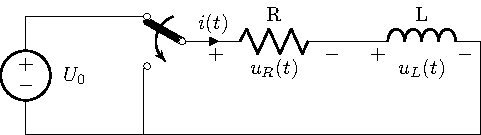
\includegraphics[width=.9\linewidth]{figs/transitorio_circuitoRL.pdf}
\end{center}
\end{frame}

\begin{frame}[label={sec:org5671cb9}]{Respuesta natural}
\begin{center}
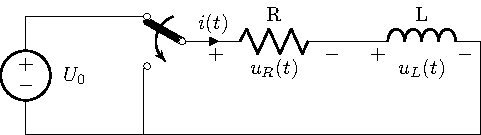
\includegraphics[width=.9\linewidth]{figs/transitorio_circuitoRL.pdf}
\end{center}

\begin{block}{Ecuaciones}
\begin{align*}
  u_R(t) + u_L(t) &= 0\\
  R i + L\diff{i}{t} &= 0
\end{align*}
\end{block}
\end{frame}

\begin{frame}[label={sec:org9500cb6}]{Respuesta natural}
\begin{block}{Solución Genérica}
\[
  i(t) = A e^{st}
\]
\end{block}

\begin{block}{Ecuación Característica}
\[
  s + \frac{R}{L} = 0 \Rightarrow s = -\frac{R}{L}
\]
\end{block}
\end{frame}

\begin{frame}[label={sec:org00c3fa1}]{Condiciones Iniciales}
\begin{itemize}
\item Analizando circuito para \(t < 0\) obtenemos  \(i(0^-) = I_0\)
\item Por otra parte, para \(t > 0\):
\end{itemize}
\begin{align*}
  i(t) &= A e^{-R/L t}\\
  i(0^+) &= A e^0 = A\\
\end{align*}

\begin{itemize}
\item Y dada la condición de continuidad, \(i(0^+) = i(0^-)\):
\end{itemize}
\begin{align*}
  A &= I_0\\
  i(t) &= I_0 e^{-R/L t}\\
\end{align*}
\end{frame}


\begin{frame}[label={sec:org2b1fc21}]{Constante de tiempo}
\begin{itemize}
\item \(\tau = \frac{L}{R}\) es la constante de tiempo (unidades [s]).
\item Ratio entre almacenamiento (\(L\)) y disipación (\(R\)).
\end{itemize}

\[
  i(t) = I_0 e^{-t/\tau}  
\]

\begin{center}
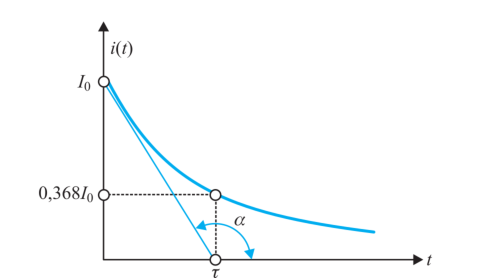
\includegraphics[width=.9\linewidth]{figs/RespuestaNatural_RL.pdf}
\end{center}
\end{frame}

\begin{frame}[label={sec:org58fb540}]{Constante de tiempo}
\begin{itemize}
\item Valores altos de \(\tau\) implican decrecimiento lento.
\item La respuesta natural \guillemotleft{}desaparece\guillemotright{} tras \(\simeq 5\tau\).
\end{itemize}

\begin{center}
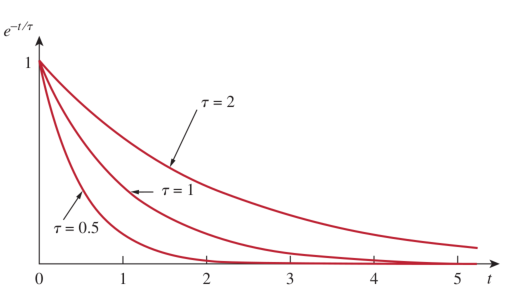
\includegraphics[width=.9\linewidth]{figs/constante_tiempo.pdf}
\end{center}
\end{frame}

\begin{frame}[label={sec:org231e2bc}]{Balance Energético}
\begin{block}{}
La energía acumulada en la bobina en \(t < 0\) se disipa en la resistencia en \(t > 0\)

\[
  W_R = \int_0^\infty R i^2(t)  \mathrm{d}t = \frac{1}{2} L I_0^2 = W_L
\]
\end{block}
\end{frame}

\begin{frame}[label={sec:orgab701a5}]{Respuesta forzada}
Cambia el funcionamiento del interruptor: en \(t > 0\) la fuente alimenta el circuito RL.
\begin{center}
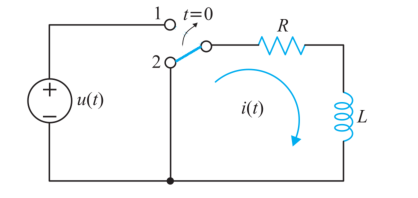
\includegraphics[width=.9\linewidth]{figs/RL_forzada.pdf}
\end{center}
\end{frame}

\begin{frame}[label={sec:orgaaa5d34}]{Respuesta forzada}
\begin{block}{Ecuaciones}
\begin{align*}
  u_R(t) + u_L(t) &= u(t)\\
  R i + L\diff{i}{t} &= U_0
\end{align*}
\end{block}

\begin{block}{Solución}
Para la solución particular se propone función análoga a la excitación (analizando circuito para \(t > 0\))
\begin{align*}
  i(t) &= i_n(t) + i_\infty(t)\\
  i_n(t) &= A e^{st}\\
  i_\infty(t) &= U_0/R\\
\end{align*}
\end{block}
\end{frame}

\begin{frame}[label={sec:org79634fd}]{Condiciones iniciales}
\begin{block}{Planteamiento General}
\begin{align*}
  i(0^+) &= i_n(0^+) + i_\infty(0^+)\\
  i(0^+) &= A + i_\infty(0^+)\\
  A &= i(0^+) - i_\infty(0^+)
\end{align*}
\end{block}
\end{frame}

\begin{frame}[label={sec:org9dc714f}]{Respuesta completa (ejemplo)}
Suponiendo que la bobina está inicialmente descargada, \(i(0^-) = 0 \Rightarrow i(0^+) = 0\)
\begin{align*}
  A &= 0 - U_0/R\\
  i(t) &= \frac{U_0}{R}(1 - e^{-\frac{t}{\tau}})  
\end{align*}

\begin{center}
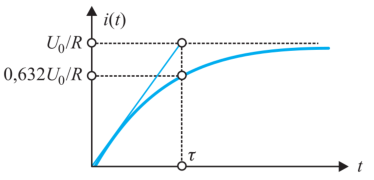
\includegraphics[width=.9\linewidth]{figs/RespuestaCompleta_RL.pdf}
\end{center}
\end{frame}


\begin{frame}[label={sec:org11046a1}]{Respuesta completa}
\begin{itemize}
\item \(i(0^+)\): corriente en la bobina, condiciones iniciales (\(i(0^-) = i(0^+)\)).
\item \(i_\infty(t)\): corriente en la bobina en régimen permanente para \(t > 0\).
\item \(i_\infty(0^+)\): corriente en la bobina en régimen permanente particularizada en \(t = 0\).
\end{itemize}

\[
i(t) = \left(i(0^+) - i_\infty(0^+)\right) e^{-t/\tau} + i_\infty(t)
\]
\end{frame}

\section{Circuito RC paralelo}
\label{sec:orgb5fbdab}

\begin{frame}[label={sec:org119a0f8}]{Circuito básico}
\begin{itemize}
\item En \(t <0\) la fuente alimenta el circuito RC (el condensador se carga).
\item En \(t = 0\) se desconecta la fuente (el condensador comienza a descargarse en la resistencia).
\end{itemize}
\begin{center}
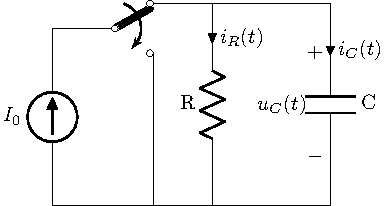
\includegraphics[width=.9\linewidth]{figs/transitorio_circuitoRC.pdf}
\end{center}
\end{frame}

\begin{frame}[label={sec:orgdb34b5a}]{Respuesta natural}
\begin{center}
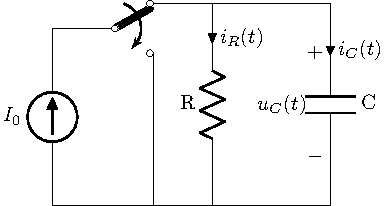
\includegraphics[width=.9\linewidth]{figs/transitorio_circuitoRC.pdf}
\end{center}

\begin{block}{Ecuaciones}
\begin{align*}
  i_R(t) + i_C(t) &= 0\\
  G u + C\diff{u}{t} &= 0
\end{align*}
\end{block}
\end{frame}

\begin{frame}[label={sec:orgf970c43}]{Respuesta natural}
\begin{block}{Solución Genérica}
\[
  u(t) = A e^{st}
\]
\end{block}

\begin{block}{Ecuación Característica}
\[
  s + \frac{G}{C} = 0 \Rightarrow s = -\frac{G}{C}
\]
\end{block}

\begin{block}{Condiciones Iniciales}
\[
  u(t) = U_0 e^{-G/C t}
\]
\end{block}
\end{frame}



\begin{frame}[label={sec:org7b91374}]{Constante de tiempo}
\begin{itemize}
\item \(\tau = \frac{C}{G}\) es la constante de tiempo (unidades [s]).
\item Ratio entre almacenamiento (\(C\)) y disipación (\(G\)).
\end{itemize}

\[
  u(t) = U_0 e^{-t/\tau}  
\]

\begin{center}
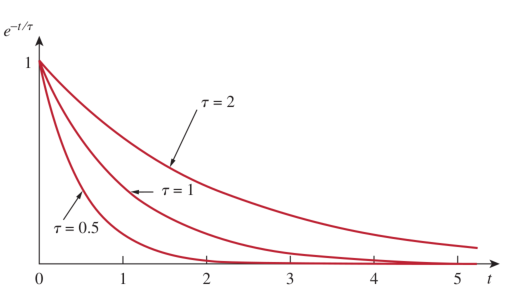
\includegraphics[width=.9\linewidth]{figs/constante_tiempo.pdf}
\end{center}
\end{frame}

\begin{frame}[label={sec:orgfd44e13}]{Balance Energético}
\begin{block}{}
La energía acumulada en el condensador en \(t < 0\) se disipa en la resistencia (conductancia) en \(t > 0\)

\[
  W_G = \int_0^\infty G u^2(t)  \mathrm{d}t = \frac{1}{2} C U_0^2 = W_C
\]
\end{block}
\end{frame}

\begin{frame}[label={sec:org84517fa}]{Respuesta completa}
\begin{itemize}
\item \(u(0^+)\): tensión en el condensador, condiciones iniciales (\(u(0^-) = u(0^+)\)).
\item \(u_\infty(t)\): tensión en el condensador en régimen permanente para \(t > 0\).
\item \(u_\infty(0^+)\): tensión en el condensador en régimen permanente particularizada en \(t = 0\).
\end{itemize}

\[
u(t) = \left(u(0^+) - u_\infty(0^+)\right) e^{-t/\tau} + u_\infty(t)
\]

\begin{block}{Ejemplo}
Suponiendo que el condensador está inicialmente descargado, \(u(0^-) = 0 \Rightarrow u(0^+) = 0\)
\begin{align*}
  A &= 0 - I_0/G\\
  u(t) &= \frac{I_0}{G}(1 - e^{-\frac{t}{\tau}})  
\end{align*}
\end{block}
\end{frame}

\section{Análisis Sistemático}
\label{sec:orgad51a22}

\begin{frame}[label={sec:orgcbd65df}]{Equivalente de Thévenin (Norton)}
\begin{center}
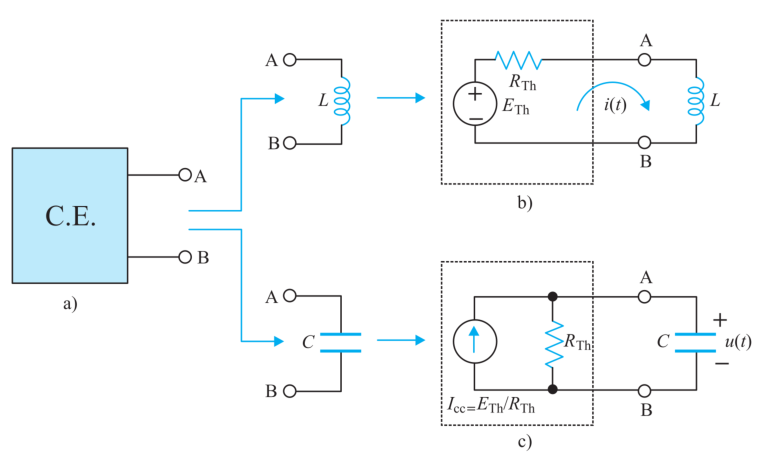
\includegraphics[width=.9\linewidth]{figs/Thevenin_PrimerOrden.pdf}
\end{center}
\end{frame}

\begin{frame}[label={sec:org2ab4a4c}]{Procedimiento General}
\begin{itemize}
\item Dibujar el circuito para \(t < 0\).
\begin{itemize}
\item Determinar variables en régimen permanente, \(u_c(t)\), \(i_L(t)\).
\item Particularizar para \(t = 0\), obteniendo \(u_c(0^-)\) o \(i_L(0^-)\).
\item Continuidad: \(u_c(0^+) = u_c(0^-)\), \(i_L(0^+) = i_L(0^-)\).
\end{itemize}
\item Dibujar el circuito para \(t > 0\).
\begin{itemize}
\item Calcular el equivalente de Thevenin (Norton) visto por el elemento de acumulación.
\item La constante de tiempo de la respuesta natural es \(\tau = \frac{L}{R_{th}}\) o \(\tau = \frac{C}{G_{th}}\).
\item Calcular las variables \(i_L(t)\) o \(u_c(t)\) en régimen permanente, obteniendo \(i_\infty(t)\) o \(u_\infty(t)\).
\item Obtener respuesta completa:
\end{itemize}
\end{itemize}
\begin{align*}
i_L(t) &= \left(i_L(0^+) - i_\infty(0^+)\right) e^{-t/\tau} + i_\infty(t)\\
u_C(t) &= \left(u_C(0^+) - u_\infty(0^+)\right) e^{-t/\tau} + u_\infty(t)\\
\end{align*}
\end{frame}


\section{Ejercicios Recomendados}
\label{sec:org0ae225e}

\begin{frame}[label={sec:orgc98985a}]{Ejercicios}
\begin{block}{FM}
Ejemplos de aplicación 4.2, 4.3, 4.4, y 4.7
\end{block}
\begin{block}{HKD}
Ejemplo 8.4, 8.6, 8.10
\end{block}
\begin{block}{AS}
Ejemplo 7.13
\end{block}
\end{frame}
\end{document}